\documentclass[dvisvgm,multi=true]{standalone}
\usepackage{mathmlcoresvg}
\begin{document}
%<figcaption><span>Figure 20: </span>Box model for the <code>msub</code> element</figcaption>
  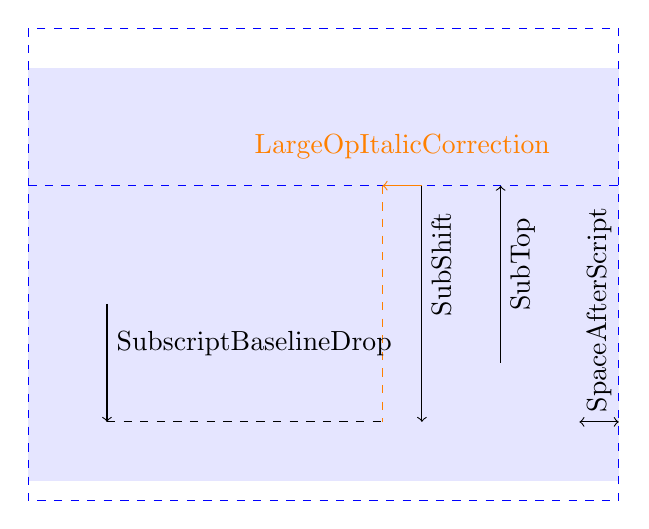
\begin{tikzpicture}[yscale=-1]

  \fill[blue!10](0,-1.5) rectangle (7.5,3.75);

  \MathMLBox{0}{0}{1}{1}{red};

  \MathMLBox{4.5}{3}{.5}{.5}{green};

  \draw[dashed,blue](0,-2) rectangle(7.5,4)
  (0,0)--(7.5,0);

   \draw[->] (5,0) -- (5,1)node[below,rotate=90]{SubShift} -- (5,3);

   \draw[orange,->] (5,0) -- (4.5,0);
   \draw[orange] (4.75, -.5) node{LargeOpItalicCorrection};
   \draw[dashed,orange] (4.5,0) -- (4.5,3);

   \draw[<-] (6,0) -- (6,1)node[below,rotate=90]{SubTop} -- (6,2.25);

   \draw[<->] (7,3) -- (7.25,3)node[right,rotate=90]{SpaceAfterScript} -- (7.5,3);

   \draw[->] (1,1.5) -- (1,2)node[right]{SubscriptBaselineDrop} -- (1,3);
   \draw[dashed] (1,3) -- (4.5,3);
\end{tikzpicture}

\end{document}
